% Provenance (never printed): the markets-and-prices strand of ../economics_series.md (grade 7). Brief:
% sources/book1/BRIEFS.md, g7-05 (the Pink Sheet was refused, so the opening chart uses BLS average prices).
% Chart data: figdata/grade-7/05-markets-and-prices (BLS average prices, eggs; FAOSTAT wheat production).
% Ledger: g7:hpai-hens-lost, g7:egg-wholesale-2022-2023, g7:russia-export-ban-2010, g7:wheat-price-2010,
% g7:fao-wheat-forecast-2010.
\chapter{Markets and Prices}\label{ch:g7:markets-and-prices}

\begin{openingchart}{Average price of a dozen large eggs in shops in the United States,
each month from January 2019 to October 2026, in dollars (no price was collected for
October 2025).}{U.S. Bureau of Labor Statistics, average \omterm{def:g7:money:price}{price} data, eggs, grade A,
large, per dozen, U.S. city average}
\begin{tikzpicture}
\begin{axis}[omtime, xmin=2019, xmax=2027, ymin=0, ymax=7,
  xtick={2019,2020,2021,2022,2023,2024,2025,2026,2027}, xlabel={Year},
  ylabel={Dollars per dozen}]
\addplot[omThm, thick] table[x=t, y=price] {figdata/grade-7/05-markets-and-prices/out/eggs_a.csv};
\addplot[omThm, thick, forget plot] table[x=t, y=price] {figdata/grade-7/05-markets-and-prices/out/eggs_b.csv};
\end{axis}
\end{tikzpicture}
\end{openingchart}

% figdata: facts (eggs_2021_12 1.79, eggs_2023_01 4.82, eggs_2023_08 2.04, eggs_peak 6.23 in 2025-03,
% eggs_last 2.32 in 2026-10)
% ledger: g7:hpai-hens-lost (more than 43 million), g7:egg-wholesale-2022-2023 (5.37 then 0.89)
For years, a dozen eggs cost about a dollar and a half in American shops. In December
2021 the \omterm{def:g7:money:price}{price} was $1.79$ dollars; in January 2023 it was $4.82$ dollars, more than two and
a half times as much. Then it fell back to $2.04$ dollars by August 2023. What happened? In 2022
a disease of birds spread through American farms, and more than 43 million egg-laying hens
were lost to it. Fewer hens meant fewer eggs, and the \omterm{def:g7:money:price}{price} shot up. As farms restocked
their flocks, eggs came back and the \omterm{def:g7:money:price}{price} fell: the wholesale \omterm{def:g7:money:price}{price}, paid by shops to
farms, went from $5.37$ dollars a dozen at the end of 2022 to $0.89$ dollars in May 2023.
The \omterm{def:g7:money:price}{price} rose again in 2024 and early 2025, to $6.23$ dollars in March 2025, and was
$2.32$ dollars in October 2026.

Nobody decided these \omterm{def:g7:money:price}{prices}: no office set them. They came out of millions of purchases
and sales. This chapter explains how a \omterm{def:g7:money:price}{price} is formed in a \omterm{def:g7:markets-and-prices:market}{market}, and what it does.

\begin{recall}
A \omterm{def:g7:money:price}{price} is an amount of \omterm{def:g7:money:money}{money} given for one unit of a good (\cref{ch:g7:money}). In an
exchange, each side gives something to the other (\cref{ch:g7:specialisation}).
\end{recall}

\section{Where buyers meet sellers}

\begin{definition}[Market]\label{def:g7:markets-and-prices:market}
A \emph{market}\index{market} is any arrangement in which buyers and sellers of a good or
service meet, in one place or at a distance, and agree on exchanges.
\end{definition}

A \omterm{def:g7:markets-and-prices:market}{market} can be a street with stalls, an auction hall where fish are sold to the highest
bidder, a shop, a website where strangers buy and sell, or a network of traders who never
meet but phone and message each other, as in the world's grain trade.

\begin{omfigure}
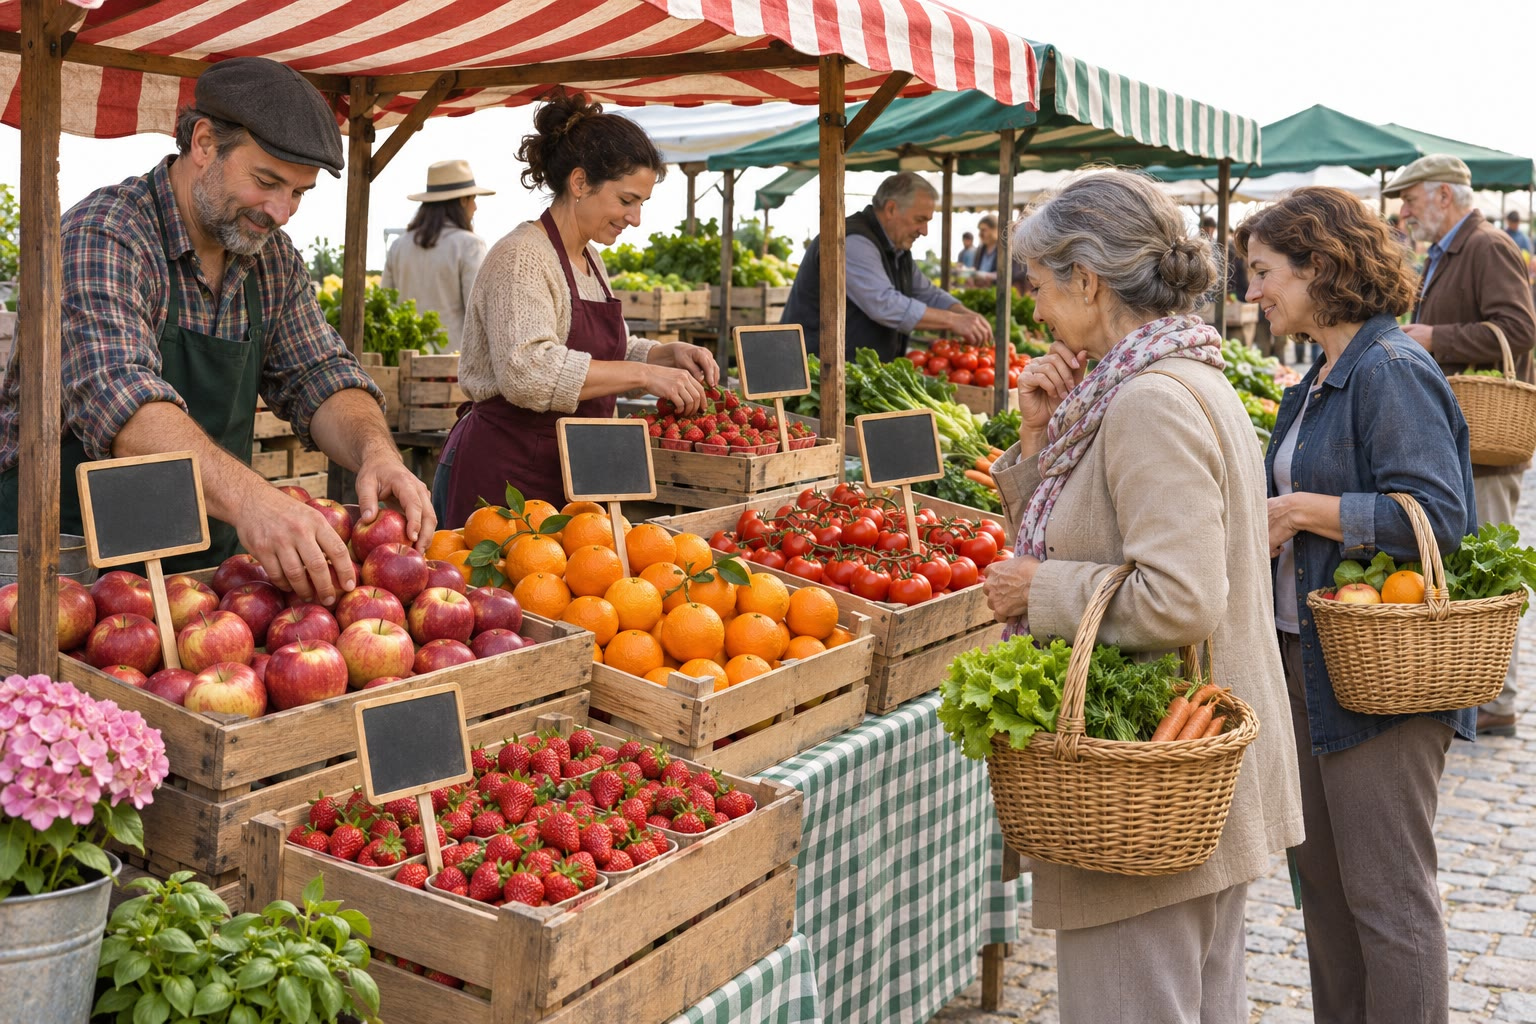
\includegraphics[width=0.55\linewidth]{images/book1/ai/g7-markets-and-prices-fruit-market.jpg}

{\small A morning \omterm{def:g7:markets-and-prices:market}{market}. Shoppers compare stalls; sellers watch what the other stalls
ask. Within an hour, the same fruit sells at almost the same \omterm{def:g7:money:price}{price} everywhere.}
\end{omfigure}

\section{The price both accept}

\begin{definition}[Market price]\label{def:g7:markets-and-prices:market-price}
The \emph{market price}\index{market price} of a good is the \omterm{def:g7:money:price}{price} at which buyers and
sellers actually exchange it in a \omterm{def:g7:markets-and-prices:market}{market}.
\end{definition}

A seller wants a high \omterm{def:g7:money:price}{price}; a buyer wants a low one. An exchange happens only at a
\omterm{def:g7:money:price}{price} that both accept. At a high \omterm{def:g7:money:price}{price}, sellers bring a lot but buyers want little, and
fruit is left unsold; sellers then lower their \omterm{def:g7:money:price}{prices}. At a low \omterm{def:g7:money:price}{price}, buyers want a lot
but sellers bring little, and buyers go home without fruit; some then offer more, and
sellers raise their \omterm{def:g7:money:price}{prices}. The \omterm{def:g7:money:price}{price} settles where the quantity that buyers want is about
the quantity that sellers offer.

\begin{example}
At an invented \omterm{def:g7:markets-and-prices:market}{market}, the table gives the kilograms of cherries that buyers want and that
sellers offer in a morning, at each \omterm{def:g7:money:price}{price}.
\begin{center}
\begin{tabular}{lccccc}
\toprule
\omterm{def:g7:money:price}{Price} (dalens per kilogram) & 2 & 3 & 4 & 5 & 6 \\
\midrule
Wanted by buyers (kg) & 100 & 80 & 60 & 40 & 20 \\
Offered by sellers (kg) & 20 & 40 & 60 & 80 & 100 \\
\bottomrule
\end{tabular}
\end{center}
At 6 dalens, 100 kg are offered and 20 wanted: 80 kg would be left. At 2 dalens, 100 kg
are wanted and 20 offered. Only at 4 dalens do the two quantities match: 60 kg are sold, at
4 dalens a kilogram.
\end{example}

\section{A price is a signal}

When the \omterm{def:g7:money:price}{price} of a good rises, it tells buyers to use less of it, and it tells sellers
to bring more. Nobody needs to know \emph{why} the \omterm{def:g7:money:price}{price} rose to react to it.

\begin{omfigure}
\begin{tikzpicture}[econ, x=1cm, y=1cm,
  box/.style={draw, rounded corners=2pt, align=center, font=\scriptsize, minimum width=3.4cm,
    minimum height=1cm}]
  \node[box, fill=omDef!25] (p) at (0,0) {the price of eggs\\rises};
  \node[box, fill=omMeth!12] (b) at (-4,-2) {buyers: eat fewer eggs,\\bake with less egg};
  \node[box, fill=omMeth!12] (s) at (4,-2) {sellers: keep old hens longer,\\bring eggs from far away};
  \draw[-{Stealth}, thick] (p) -- node[above left, font=\scriptsize] {use less} (b);
  \draw[-{Stealth}, thick] (p) -- node[above right, font=\scriptsize] {bring more} (s);
  \node[box, fill=black!8] (r) at (0,-3.6) {the shortage shrinks};
  \draw[-{Stealth}] (b) -- (r);
  \draw[-{Stealth}] (s) -- (r);
\end{tikzpicture}

{\small A \omterm{def:g7:money:price}{price} rise sends two messages at once: one to buyers, one to sellers. Both
reduce the gap between what is wanted and what is offered.}
\end{omfigure}

\begin{model}{Prices as signals}
\assumes Many buyers and many sellers of a good; its \omterm{def:g7:money:price}{price} is free to move.
\predicts After a bad harvest, the \omterm{def:g7:money:price}{price} rises; buyers use less, and other growers and
stores bring more; when supplies come back, the \omterm{def:g7:money:price}{price} falls.
\tested The egg \omterm{def:g7:money:price}{price} after the loss of laying hens in 2022 (the opening chart); the wheat
\omterm{def:g7:money:price}{price} after the Russian harvest failure of 2010 (the record below).
\breaks When a \omterm{def:g7:money:price}{price} is held fixed, by a rule or a law, it cannot send its signal
(the last section, and \cref{ch:g9:price-controls-taxes-subsidies}); when a single seller
sets the \omterm{def:g7:money:price}{price} (\cref{ch:g8:competition-and-monopoly-first-look}).
\end{model}

\begin{omchart}{Wheat production in Russia, Kazakhstan and Ukraine, 2005--2015, in millions
of tonnes.}{Food and Agriculture Organization of the United Nations, FAOSTAT, crops: wheat,
production}
\begin{tikzpicture}
\begin{axis}[omtime, xmin=2005, xmax=2015, ymin=0, ymax=70,
  xtick={2005,2007,2009,2011,2013,2015}, xlabel={Year},
  ylabel={Millions of tonnes},
  legend style={at={(0.5,-0.2)}, anchor=north, legend columns=3}]
\pgfplotsforeachungrouped \col in {rus, kaz, ukr} {
  \addplot table[x=year, y=\col] {figdata/grade-7/05-markets-and-prices/out/black_sea_wheat.csv};
}
\legend{Russia, Kazakhstan, Ukraine}
\end{axis}
\end{tikzpicture}
\end{omchart}

\begin{record}[The 2010 wheat harvest]
% figdata: facts (rus_2009 61.7, rus_2010 41.5, kaz_2009 17.1, kaz_2010 9.6, ukr_2009 20.9, ukr_2010 16.9,
% world_2009 684.7, world_2010 653.7, world_2011 698.0, world_area_2010 216.7, world_area_2011 220.8)
% ledger: g7:wheat-price-2010, g7:fao-wheat-forecast-2010, g7:russia-export-ban-2010
In the summer of 2010, a severe drought hit the wheat fields of Russia,
Kazakhstan and Ukraine. Russia harvested $41.5$ million tonnes of wheat, against $61.7$
million the year before; Kazakhstan $9.6$ against $17.1$. In early August, the Food and Agriculture
Organization of the United Nations cut its forecast of the world harvest from 676 to 651 million tonnes. From June to
early August, the world \omterm{def:g7:money:price}{price} of wheat almost doubled. On 5 August, Russia's government
decided to ban its \omterm{def:g6:a-connected-world:export}{exports} of wheat and other grains from 15 August to 31 December 2010.
The ban kept the grain at home, so inside Russia the \omterm{def:g7:money:price}{price} could not send the world's
signal to Russian buyers and growers. Elsewhere, the model predicts the rest: the higher
\omterm{def:g7:money:price}{price} told mills, bakers and farmers who feed grain to animals to use less, and told growers
everywhere to sow more. In 2011, the world's wheat fields grew from $216.7$ to $220.8$ million
hectares, the world harvested 698 million tonnes, more than before the drought, and Russia's
harvest recovered to $56.2$ million tonnes. Part of the recovery was the return of normal
weather; the \omterm{def:g7:money:price}{price}'s part shows in the 4 million more hectares sown.
\end{record}

\begin{measure}[A world price]
The ``world \omterm{def:g7:money:price}{price}'' of wheat is not one number fixed somewhere. It is the \omterm{def:g7:money:price}{price} of a
standard quality of wheat, quoted every day at the main ports or on exchanges where large
traders buy and sell. \omterm{def:g7:money:price}{Prices} in each country differ from it by the cost of transport, by
taxes on \omterm{def:g6:a-connected-world:import}{imports} and \omterm{def:g6:a-connected-world:export}{exports}, and by quality. A rise in the world \omterm{def:g7:money:price}{price} spreads to the
countries that trade, more slowly to those that trade little.
\end{measure}

\section{What a price knows}

Think of everything that lies behind the \omterm{def:g7:money:price}{price} of eggs: the number of hens on thousands of
farms, the \omterm{def:g7:money:price}{price} of their feed, the disease, the weather, the cost of trucks, the tastes of
millions of shoppers. No one person knows all this, and no office collects it. Yet the \omterm{def:g7:money:price}{price}
sums it up. A baker who sees the \omterm{def:g7:money:price}{price} of eggs double does not need to know about the
disease: the \omterm{def:g7:money:price}{price} alone tells her that eggs are scarce now, and that it pays to use fewer.
A farmer in another region does not need to know who is short of eggs: the \omterm{def:g7:money:price}{price} tells him
that it pays to keep his hens laying and to sell further away. Through \omterm{def:g7:money:price}{prices}, millions of
people who never meet adjust to each other, and the scarce good goes where it is most wanted.

\section{When a price cannot move}

\begin{definition}[Shortage]\label{def:g7:markets-and-prices:shortage}
A \emph{shortage}\index{shortage} is the situation in which, at the going \omterm{def:g7:money:price}{price}, the
quantity that buyers want is larger than the quantity that sellers offer.
\end{definition}

\begin{definition}[Market surplus]\label{def:g7:markets-and-prices:market-surplus}
A \emph{market surplus}\index{market surplus} is the situation in which, at the going \omterm{def:g7:money:price}{price},
the quantity that sellers offer is larger than the quantity that buyers want.
\end{definition}

In a \omterm{def:g7:markets-and-prices:market}{market} where the \omterm{def:g7:money:price}{price} can move, a \omterm{def:g7:markets-and-prices:shortage}{shortage} or a \omterm{def:g7:markets-and-prices:market-surplus}{market surplus} does not last: the
\omterm{def:g7:money:price}{price} rises or falls until the two quantities match. If the \omterm{def:g7:money:price}{price} cannot move --- because a
rule fixes it, or a seller keeps the same \omterm{def:g7:money:price}{price} on a sign --- the gap remains. In the example
of the cherries, a \omterm{def:g7:money:price}{price} fixed at 3 dalens would leave a \omterm{def:g7:markets-and-prices:shortage}{shortage} of $80 - 40 = 40$
kilograms: buyers would queue, the first to arrive would get cherries, and the others none.
A \omterm{def:g7:money:price}{price} fixed at 5 dalens would leave a \omterm{def:g7:markets-and-prices:market-surplus}{market surplus} of $80 - 40 = 40$ kilograms of unsold
cherries.

\section{Exercises}

\begin{exercise}[$\star$]\label{exo:g7:markets-and-prices:1}
Use the wheat chart. About how much wheat did Russia produce in 2009, and in 2010?
\end{exercise}

\begin{exercise}[$\star$]\label{exo:g7:markets-and-prices:2}
At a \omterm{def:g7:money:price}{price} of 3 dalens, buyers want 120 kg of plums and sellers offer 80 kg. Is there a
\omterm{def:g7:markets-and-prices:shortage}{shortage} or a \omterm{def:g7:markets-and-prices:market-surplus}{market surplus}, and of how many kilograms?
\end{exercise}

\begin{exercise}[$\star$]\label{exo:g7:markets-and-prices:3}
At a \omterm{def:g7:money:price}{price} of 6 dalens, buyers want 50 kg of plums and sellers offer 90 kg. Is there a
\omterm{def:g7:markets-and-prices:shortage}{shortage} or a \omterm{def:g7:markets-and-prices:market-surplus}{market surplus}, and of how many kilograms?
\end{exercise}

\begin{exercise}[$\star$]\label{exo:g7:markets-and-prices:4}
Use the opening chart. Did the \omterm{def:g7:money:price}{price} of eggs rise or fall from January 2023 to August 2023?
Give the two \omterm{def:g7:money:price}{prices} from the text.
\end{exercise}

\begin{exercise}[$\star\star$]\label{exo:g7:markets-and-prices:5}
A late frost destroys half of a region's strawberries. Predict, with the model ``\omterm{def:g7:money:price}{Prices} as
signals'', what happens to the \omterm{def:g7:money:price}{price} of strawberries and to the quantity sold. Explain.
\end{exercise}

\begin{exercise}[$\star\star$]\label{exo:g7:markets-and-prices:6}
A large new orchard doubles the apples on sale in a town. Predict what happens to the \omterm{def:g7:money:price}{price}
and to the quantity sold. Explain.
\end{exercise}

\begin{exercise}[$\star\star$]\label{exo:g7:markets-and-prices:7}
The wholesale \omterm{def:g7:money:price}{price} of eggs was $5.37$ dollars a dozen at the end of 2022 and $0.89$ dollars
in May 2023. Compute the fall in percent, rounded to one decimal.
\end{exercise}

\begin{exercise}[$\star\star$]\label{exo:g7:markets-and-prices:8}
Use the values in the record box. (a) How much less wheat did the world harvest in 2010 than
in 2009? (b) How much more in 2011 than in 2010? (c) What part of the model does (b) fit?
\end{exercise}

\begin{exercise}[$\star\star$]\label{exo:g7:markets-and-prices:9}
Describe an observation that would contradict the model ``\omterm{def:g7:money:price}{Prices} as signals''.
\end{exercise}

\begin{exercise}[$\star\star\star$]\label{exo:g7:markets-and-prices:10}
After a bad harvest, a town keeps the \omterm{def:g7:money:price}{price} of potatoes at 1 dalen a kilogram. At that
\omterm{def:g7:money:price}{price}, households want 9\,000 kg a week, but only 6\,000 kg are offered. Each household
buys 3 kg. (a) What is the \omterm{def:g7:markets-and-prices:shortage}{shortage}? (b) How many households go without potatoes each week?
(c) If the potatoes are sold to the first in the queue, what might people do?
\end{exercise}

\begin{exercise}[$\star\star\star$]\label{exo:g7:markets-and-prices:11}
At a fish auction, ten buyers each want one box of fish. The highest \omterm{def:g7:money:price}{price} each is willing
to pay is: 30, 28, 27, 25, 24, 22, 20, 18, 15, 12 dalens. There are 4 boxes. (a) If the \omterm{def:g7:money:price}{price}
rises until only 4 buyers are left, between which two values must it end? (b) What if there
were 6 boxes?
\end{exercise}

\begin{exercise}[$\star\star\star$]\label{exo:g7:markets-and-prices:12}
The opening chart shows the average \omterm{def:g7:money:price}{price} of eggs. Name two questions about who bore the
higher \omterm{def:g7:money:price}{price} that the chart cannot answer, and say what data would answer one of them.
\end{exercise}

\section{Problem: A Frost in the Orchards}

\begin{problem}[{Weekend problem --- the Brenmoor apple market before a frost, the new
price after it, and a price fixed by the town}]
\label{pb:g7:markets-and-prices:1}
Everything in this problem is invented. The table gives the tonnes of apples that the
households of Brenmoor want each week, and that the orchards offer, at each \omterm{def:g7:money:price}{price} in dalens
per kilogram.
\begin{center}
\begin{tabular}{lccccc}
\toprule
\omterm{def:g7:money:price}{Price} (dalens per kg) & 1 & 2 & 3 & 4 & 5 \\
\midrule
Wanted (tonnes a week) & 50 & 40 & 30 & 20 & 10 \\
Offered before the frost (tonnes a week) & 10 & 20 & 30 & 40 & 50 \\
\bottomrule
\end{tabular}
\end{center}

\medskip
\noindent\textbf{Part I --- Before the frost.}
\begin{enumerate}
  \item At 2 dalens, is there a \omterm{def:g7:markets-and-prices:shortage}{shortage} or a \omterm{def:g7:markets-and-prices:market-surplus}{market surplus}? Of how many tonnes?
  \item At 5 dalens, is there a \omterm{def:g7:markets-and-prices:shortage}{shortage} or a \omterm{def:g7:markets-and-prices:market-surplus}{market surplus}? Of how many tonnes?
  \item What are the \omterm{def:g7:markets-and-prices:market-price}{market price} and the quantity sold?
  \item How many dalens do households spend on apples each week? (A tonne is 1\,000 kg.)
\end{enumerate}

\medskip
\noindent\textbf{Part II --- The frost.} A frost destroys half of the blossoms: at every \omterm{def:g7:money:price}{price},
the orchards now offer half as many apples as before.
\begin{enumerate}[resume]
  \item Write the new row of quantities offered.
  \item What are the new \omterm{def:g7:markets-and-prices:market-price}{market price} and quantity sold?
  \item Compute the \omterm{def:g6:reading-economic-charts:rate-of-change}{rate of change} of the \omterm{def:g7:money:price}{price} and of the quantity sold, in percent.
  \item Explain how the new \omterm{def:g7:money:price}{price} tells households and other orchards what to do.
\end{enumerate}

\medskip
\noindent\textbf{Part III --- A fixed price.} The town decides that apples must not cost more
than 3 dalens a kilogram.
\begin{enumerate}[resume]
  \item After the frost, how many tonnes are wanted and how many offered at 3 dalens?
  \item What is the \omterm{def:g7:markets-and-prices:shortage}{shortage}, in kilograms?
  \item Each household buys 2 kg a week. How many households go without apples each week?
  \item Who gets the apples now? Name one thing that may happen that did not happen when the
        \omterm{def:g7:money:price}{price} could move.
\end{enumerate}
\end{problem}
